\documentclass[11pt,a4paper]{article}

\usepackage[utf8]{inputenc}
\usepackage[margin=18mm]{geometry}
\usepackage{graphicx}
\usepackage{booktabs}
\usepackage{amsmath,amssymb}
\usepackage{hyperref}
\usepackage{xcolor}
\usepackage{listings}
\usepackage{caption}
\usepackage{float}
\usepackage{fancyhdr}

\definecolor{uormaroon}{HTML}{7B1E33}
\definecolor{uorgold}{HTML}{F2B705}
\definecolor{codegray}{HTML}{F1F5F9}
\definecolor{codeborder}{HTML}{CBD5E1}

\hypersetup{
    colorlinks=true,
    linkcolor=uormaroon,
    filecolor=uormaroon,      
    urlcolor=uormaroon,
    pdftitle={SmartHall AI — Project Report},
    pdfauthor={D.M.S.N.H. Dissanayake},
    pdfsubject={EC4307 Web Application Development}
}

\pagestyle{fancy}
\fancyhf{}
\fancyhead[L]{\small \textbf{SmartHall AI} — University of Ruhuna (UOR-EFAC)}
\fancyhead[R]{\small EC4307 Web Application Development}
\fancyfoot[L]{\small Faculty of Engineering}
\fancyfoot[R]{\small Page \thepage}

\lstset{
    backgroundcolor=\color{codegray},
    basicstyle=\ttfamily\footnotesize,
    breaklines=true,
    frame=single,
    rulecolor=\color{codeborder},
    captionpos=b,
    numbers=left,
    numberstyle=\tiny\color{gray}
}

\begin{document}

% ----------------- TITLE & COVER -----------------
\begin{titlepage}
    \centering
    \vspace*{1cm}
    {\Large \textbf{FACULTY OF ENGINEERING $\cdot$ UNIVERSITY OF RUHUNA}}\\[0.3cm]
    {\large Department of Electrical and Information Engineering $\cdot$ Hapugala, Galle}\\[1.5cm]

    {\color{uormaroon}\hrule height 2pt}\vspace{0.8cm}
    {\Huge \textbf{SmartHall AI}}\\[0.4cm]
    {\Large \textbf{An Intelligent University Hall Allocation, Campus Navigation, and Multimodal AI Permission Letter Verification System}}\\[0.8cm]
    {\color{uormaroon}\hrule height 2pt}\vspace{1.5cm}

    \textbf{Course Module:} EC4307 — Web Application Development\\[0.3cm]
    \textbf{Academic Year:} 2026\\[1.5cm]

    \begin{tabular}{rl}
        \textbf{Author / Candidate:} & D.M.S.N.H. Dissanayake \\
        \textbf{Registration No.:} & EG/2022/5574 \\
        \textbf{GitHub Repository:} & \href{https://github.com/Cognix-0/Smart-Hall-UOR-EFAC}{Cognix-0/Smart-Hall-UOR-EFAC} \\
        \textbf{Technology Stack:} & Node.js, Express 5, EJS, MySQL 8, Claude Opus, Gemini Flash
    \end{tabular}

    \vfill
    {\large \today}
\end{titlepage}

% ----------------- EXECUTIVE SUMMARY -----------------
\section*{Executive Summary}
\addcontentsline{toc}{section}{Executive Summary}

\textbf{SmartHall AI} is a production-grade university hall allocation and campus navigation web platform built specifically to resolve the logistical friction of venue scheduling at the Faculty of Engineering, University of Ruhuna (UOR-EFAC). Prior to SmartHall AI, batch representatives, student societies, and university administrators relied on fragmented WhatsApp groups, manual spreadsheets, and physical paper permission letters to manage lecture halls and auditorium venues. This traditional approach resulted in frequent scheduling clashes, inefficient hall utilization, lost directions for junior batches, and multi-day delays in obtaining booking approvals.

SmartHall AI replaces this manual overhead with an automated, rule-governed web application featuring:
\begin{enumerate}
    \item \textbf{Algorithmic Hall Auto-Allocation} solving constrained bin-packing for lectures across all academic batches without room clashes.
    \item \textbf{Multimodal AI Letter Verification} using the Claude Opus API to check scanned society booking permission letters against 6 administrative approval criteria.
    \item \textbf{Automated PDF Timetable Ingestion} with Python coordinate-based extraction that maps official faculty timetable PDFs into live database records.
    \item \textbf{Dedicated Role-Based User Interfaces} tailored for Faculty Administrators, Cohort Batch Reps, and Society Presidents.
    \item \textbf{Natural Language Chatbot} providing instant database-backed answers and walking directions for mobile users.
    \item \textbf{Intentional High-Contrast Dark UI} designed for low-light lecture halls, low latency, and zero framework bloat.
\end{enumerate}

\newpage
\tableofcontents
\newpage

% ----------------- SECTION 1 -----------------
\section{Project Motivation \& Real-World Problem Statement}

\subsection{The Operational Problem at UOR-EFAC}
The Faculty of Engineering at the University of Ruhuna houses over 1,000 undergraduate engineering students across multiple academic batches (e.g., 25th, 26th, 27th, 28th batches) and diverse engineering disciplines. The physical campus infrastructure includes several major lecture halls, computer laboratories, drawing offices, and an auditorium:

\begin{table}[H]
    \centering
    \caption{Key Physical Teaching Venues at UOR-EFAC}
    \begin{tabular}{lllr}
        \toprule
        \textbf{Code} & \textbf{Venue Name} & \textbf{Building Location} & \textbf{Capacity} \\
        \midrule
        \textbf{MLT} & Main Lecture Theatre & Administration Building, Ground floor & 250 seats \\
        \textbf{LH1} & Lecture Hall 1 & Lecture Hall Complex, Ground floor & 180 seats \\
        \textbf{LH2} & Lecture Hall 2 & Lecture Hall Complex, 1st floor & 130 seats \\
        \textbf{ECC} & Electrical Computer Centre & EIE Department, 2nd floor & 90 seats \\
        \textbf{NCC} & New Computer Centre & Computer Centre Building, Ground floor & 120 seats \\
        \textbf{OCC} & Old Computer Centre & Computer Centre Building, Ground floor & 80 seats \\
        \textbf{DO}  & Drawing Office & Civil Engineering Building, 1st floor & 70 seats \\
        \textbf{AUD} & Faculty Auditorium & Main Auditorium Complex & 400 seats \\
        \bottomrule
    \end{tabular}
\end{table}

Managing these shared physical facilities previously suffered from three critical bottlenecks:
\begin{enumerate}
    \item \textbf{Double Bookings \& Scheduling Conflicts:} When batch representatives rescheduled lectures or when societies planned evening workshops, manual coordination led to simultaneous bookings in the same room.
    \item \textbf{Student Navigation \& Awareness:} Incoming and junior students often struggled to locate venues spread across multiple faculty complexes.
    \item \textbf{Paper-Based Bureaucracy:} Student societies had to draft physical letters, obtain the signature of an academic staff counselor, deliver the document to the Deputy Registrar / Assistant Registrar for approval, and wait days for verification.
\end{enumerate}

% ----------------- SECTION 2 -----------------
\section{Technical Architecture \& Stack}

SmartHall AI is designed as a server-side rendered (SSR) monolithic application prioritizing performance, security, and maintainability.

\begin{table}[H]
    \centering
    \caption{System Technology Stack}
    \begin{tabular}{lp{5cm}p{7cm}}
        \toprule
        \textbf{Layer} & \textbf{Technologies} & \textbf{Rationale} \\
        \midrule
        \textbf{Backend} & Node.js (v20+ LTS), Express 5 & Asynchronous, non-blocking I/O ideal for concurrent web traffic and quick database queries. \\
        \textbf{Database} & MySQL 8.0, \texttt{mysql2} & Strict relational schema, foreign key cascade constraints, compound unique keys to prevent double bookings. \\
        \textbf{Rendering} & EJS (Embedded JavaScript) & High-speed server-side rendering, semantic HTML output, and shared partials without heavy client bundles. \\
        \textbf{Styling} & Vanilla Modern CSS & Custom CSS variables, glassmorphic modals, flex/grid layouts, responsive typography, and native dark mode. \\
        \textbf{AI Engine} & Claude Opus \& Gemini Flash & Multimodal permission letter inspection and conversational chatbot query parsing. \\
        \textbf{PDF Engine} & Python 3 with \texttt{pypdf} & Precise bounding-box and coordinate-based extraction of faculty timetable matrices. \\
        \textbf{Security} & \texttt{bcryptjs}, \texttt{express-session} & Cryptographic password hashing (salt rounds = 10) and secure server-side session management. \\
        \bottomrule
    \end{tabular}
\end{table}

% ----------------- SECTION 3 -----------------
\section{Comprehensive CRUD Matrix \& Database Integrity}

\begin{table}[H]
    \centering
    \caption{System Entity CRUD Operations}
    \small
    \begin{tabular}{p{2.5cm}p{3cm}p{3.5cm}p{3cm}p{2.5cm}}
        \toprule
        \textbf{Entity} & \textbf{Create (C)} & \textbf{Read (R)} & \textbf{Update (U)} & \textbf{Delete (D)} \\
        \midrule
        \textbf{Halls} & Admin form with capacity and photo & Public list, availability board, and directions & Edit capacity, directions, or photo & Cascades bookings and unplaced slots \\
        \textbf{Batches} & Create cohort with student headcount & Batches list and student count cards & Modify name and official headcount & Cascades lectures \\
        \textbf{Time Slots} & Daily slot definitions (start/end) & Daily schedule grid & Adjust period timings with checks & Validates active dependencies \\
        \textbf{Lectures} & Manual add or CSV/PDF ingestion & Weekly batch grid and right-now card & Change day, slot, subject, or hall & Custom modal confirmation \\
        \textbf{PDF Timetables} & 1-click coordinate matrix parser & In-browser PDF view and download & Replace batch schedule & Modal confirmed cleanup \\
        \textbf{Bookings} & Rep booking or Society with letter & Filterable bookings table and preview & Approve, reject, or revoke & Immediate hall release \\
        \textbf{Users} & Bcrypt registration with role binding & User directory with role indicators & Role elevation and batch mapping & Preserves audit history \\
        \bottomrule
    \end{tabular}
\end{table}

\subsection{Relational Integrity Constraints}
Rather than relying solely on application-layer logic, SmartHall AI delegates scheduling rules to MySQL 8.0 database-level constraints:
\begin{itemize}
    \item \texttt{UNIQUE KEY one\_class\_per\_batch (batch\_id, day\_of\_week, time\_slot\_id)}: Mechanically impossible for a batch to have two scheduled classes simultaneously.
    \item \texttt{UNIQUE KEY one\_class\_per\_hall (hall\_id, day\_of\_week, time\_slot\_id)}: Physically impossible for two lectures to share the same hall in the same teaching block.
    \item \texttt{CHECK (end\_at > start\_at)}: Chronological sanity checks on all one-off events.
\end{itemize}

% ----------------- SECTION 4 -----------------
\section{Advanced Engineering \& Constrained Optimization}

\subsection{Mathematical Formulation of Best-Fit Hall Allocation}
When an administrator uploads an unassigned master timetable, SmartHall AI executes a constrained combinatorial optimization algorithm (\texttt{src/allocate.js}):

Let $E = \{e_1, e_2, \dots, e_n\}$ denote the set of unplaced timetable lecture entries, where each entry $e \in E$ is defined by:
\begin{itemize}
    \item $d(e) \in \{1, 2, 3, 4, 5\}$: assigned day of the week,
    \item $s(e) \in S$: assigned daily time slot,
    \item $c(e) \in \mathbb{N}$: enrolled batch student headcount.
\end{itemize}

Let $H = \{h_1, h_2, \dots, h_m\}$ be the set of available campus lecture halls, where each hall $h \in H$ possesses a seating capacity $K(h) \in \mathbb{N}$, and binary availability $A(h, d, s) \in \{0, 1\}$ indicating whether hall $h$ is unoccupied at day $d$ and slot $s$.

\noindent \textbf{Objective Function:}
\begin{equation}
    \min \sum_{e \in E} \sum_{h \in H} x_{e, h} \cdot \Big( K(h) - c(e) \Big)
\end{equation}

\noindent \textbf{Subject to:}
\begin{align}
    x_{e, h} = 1 &\implies K(h) \ge c(e), \quad \forall e \in E, \; \forall h \in H \quad &\text{(Capacity Feasibility)} \\
    \sum_{e \in E : d(e)=d, s(e)=s} x_{e, h} &\le A(h, d, s), \quad \forall h \in H, \; \forall d, s \quad &\text{(Conflict Exclusion)} \\
    \sum_{h \in H} x_{e, h} &\le 1, \quad \forall e \in E \quad &\text{(Unitary Assignment)}
\end{align}
where $x_{e, h} \in \{0, 1\}$ is the binary decision variable indicating whether lecture $e$ is allocated to hall $h$. SmartHall AI employs a greedy hardest-first heuristic: cohorts are sorted in descending order of $c(e)$, fitting each into the minimum adequate hall ($K(h) \ge c(e)$) to conserve large auditoriums (MLT, AUD) for major batches.

\subsection{Automated PDF Timetable Ingestion Engine}
Official faculty timetables (e.g., \texttt{9AxgTxnvgl0yADgsUzyUlvnY7uYnmrXrhK8mezyM.pdf}) are parsed via a Python pipeline (\texttt{src/parsePdf.py}):
\begin{enumerate}
    \item Extracts 2D geometric coordinates $(x, y)$ of text elements to place entries into exact Monday--Friday columns and 1-hour time blocks (\texttt{08:30--09:30} to \texttt{16:30--17:30}).
    \item Expands course shorthand abbreviations from Page 2 notes (e.g., \texttt{EC5205} $\to$ \textit{"Operating System and Network Programming"}).
    \item Normalizes faculty room shorthand (e.g., \texttt{[LT1]} $\to$ \texttt{LH1}, \texttt{[CC]} $\to$ \texttt{OCC}).
    \item One-click web interface automatically populates MySQL records and publishes the downloadable official PDF.
\end{enumerate}

\subsection{Multimodal AI Permission Letter Verification}
Society bookings require an official permission letter. SmartHall AI connects to the Claude Opus API with structured vision schema to verify:
\begin{enumerate}
    \item Addressed to the \textbf{Deputy Registrar, Faculty of Engineering}.
    \item Routed \textbf{Through the academic staff counselor}.
    \item Organization name matches the authenticated president.
    \item Requested venue and date boundaries match the form submission.
    \item Visual presence of staff counselor and approval signatures.
\end{enumerate}

% ----------------- SECTION 5 -----------------
\section{Intelligent Chatbot Architecture}
The chatbot combines a deterministic regex parser with a Gemini Flash LLM fallback:
\begin{itemize}
    \item \textbf{Regex Parser (\texttt{src/chatbot.js}):} Extracts date (today, tomorrow, dates), time (12h/24h), and headcount (e.g., \textit{"120 students"}) with zero API latency.
    \item \textbf{Live SQL Query:} Queries both timetable and booking tables to locate free halls matching capacity constraints.
    \item \textbf{Contextual Walking Directions:} Appends door-to-door wayfinding instructions (e.g., \textit{"LH1 — Lecture Hall Complex, turn right after the stairs"}).
    \item \textbf{Gemini Flash Fallback:} Answers conversational or non-standard inquiries within strict faculty knowledge bounds.
\end{itemize}

% ----------------- SECTION 6 -----------------
\section{UI/UX Design Philosophy: High-Contrast Dark Interface}
The dark visual theme (\texttt{\#0f1117} background, \texttt{\#181b24} raised surface, \texttt{\#7b1e33} maroon, \texttt{\#f2b705} gold, \texttt{\#22c55e} emerald) was an intentional HCI design choice:
\begin{enumerate}
    \item \textbf{Low-Light Lecture Theatre Comfort:} Eliminates pupil strain in darkened presentation halls.
    \item \textbf{Outdoor High-Contrast Legibility:} Saturated accent colors remain legible in bright outdoor campus sunlight.
    \item \textbf{OLED Battery Conservation:} Reduces battery drain on student smartphones during 8-hour university days.
    \item \textbf{Tactile Signplate Badges:} Hall codes mirror the physical metal doorplates on campus doors.
    \item \textbf{Sub-100ms Load Times:} Zero client-side framework bloat ensures instant loading on spotty campus Wi-Fi.
\end{enumerate}

% ----------------- SECTION 7: ROLE-BASED UIS -----------------
\newpage
\section{Dedicated Role-Based User Interfaces}

To eliminate operational friction and cognitive overload, SmartHall AI replaces generic monolithic dashboards with \textbf{specialized, role-tailored workspaces} for each authenticated persona: \textbf{System Administrator}, \textbf{Batch Representative (Rep)}, and \textbf{Society President}.

\subsection{Faculty Administrator Control Center (\texttt{/admin})}
Central command for the Faculty Timetable Committee, Assistant Registrar, and Dean's Office (\texttt{admin@smarthall.test}):
\begin{itemize}
    \item \textbf{Live Stat Monitor:} Real-time tiles showing pending booking reviews, unplaced lectures, weekly master sessions, and campus halls.
    \item \textbf{One-Click Action Toolbar:} Quick access to Timetable Setup, Batches \& Counts, Time Slots, and User Directory.
    \item \textbf{Auto-Allocation Engine:} Dispatches constrained bin-packing to resolve unassigned lectures in 1 click.
    \item \textbf{New Semester Reset:} Modal-protected utility for wiping expired schedules per batch or across the faculty.
\end{itemize}

\begin{figure}[H]
    \centering
    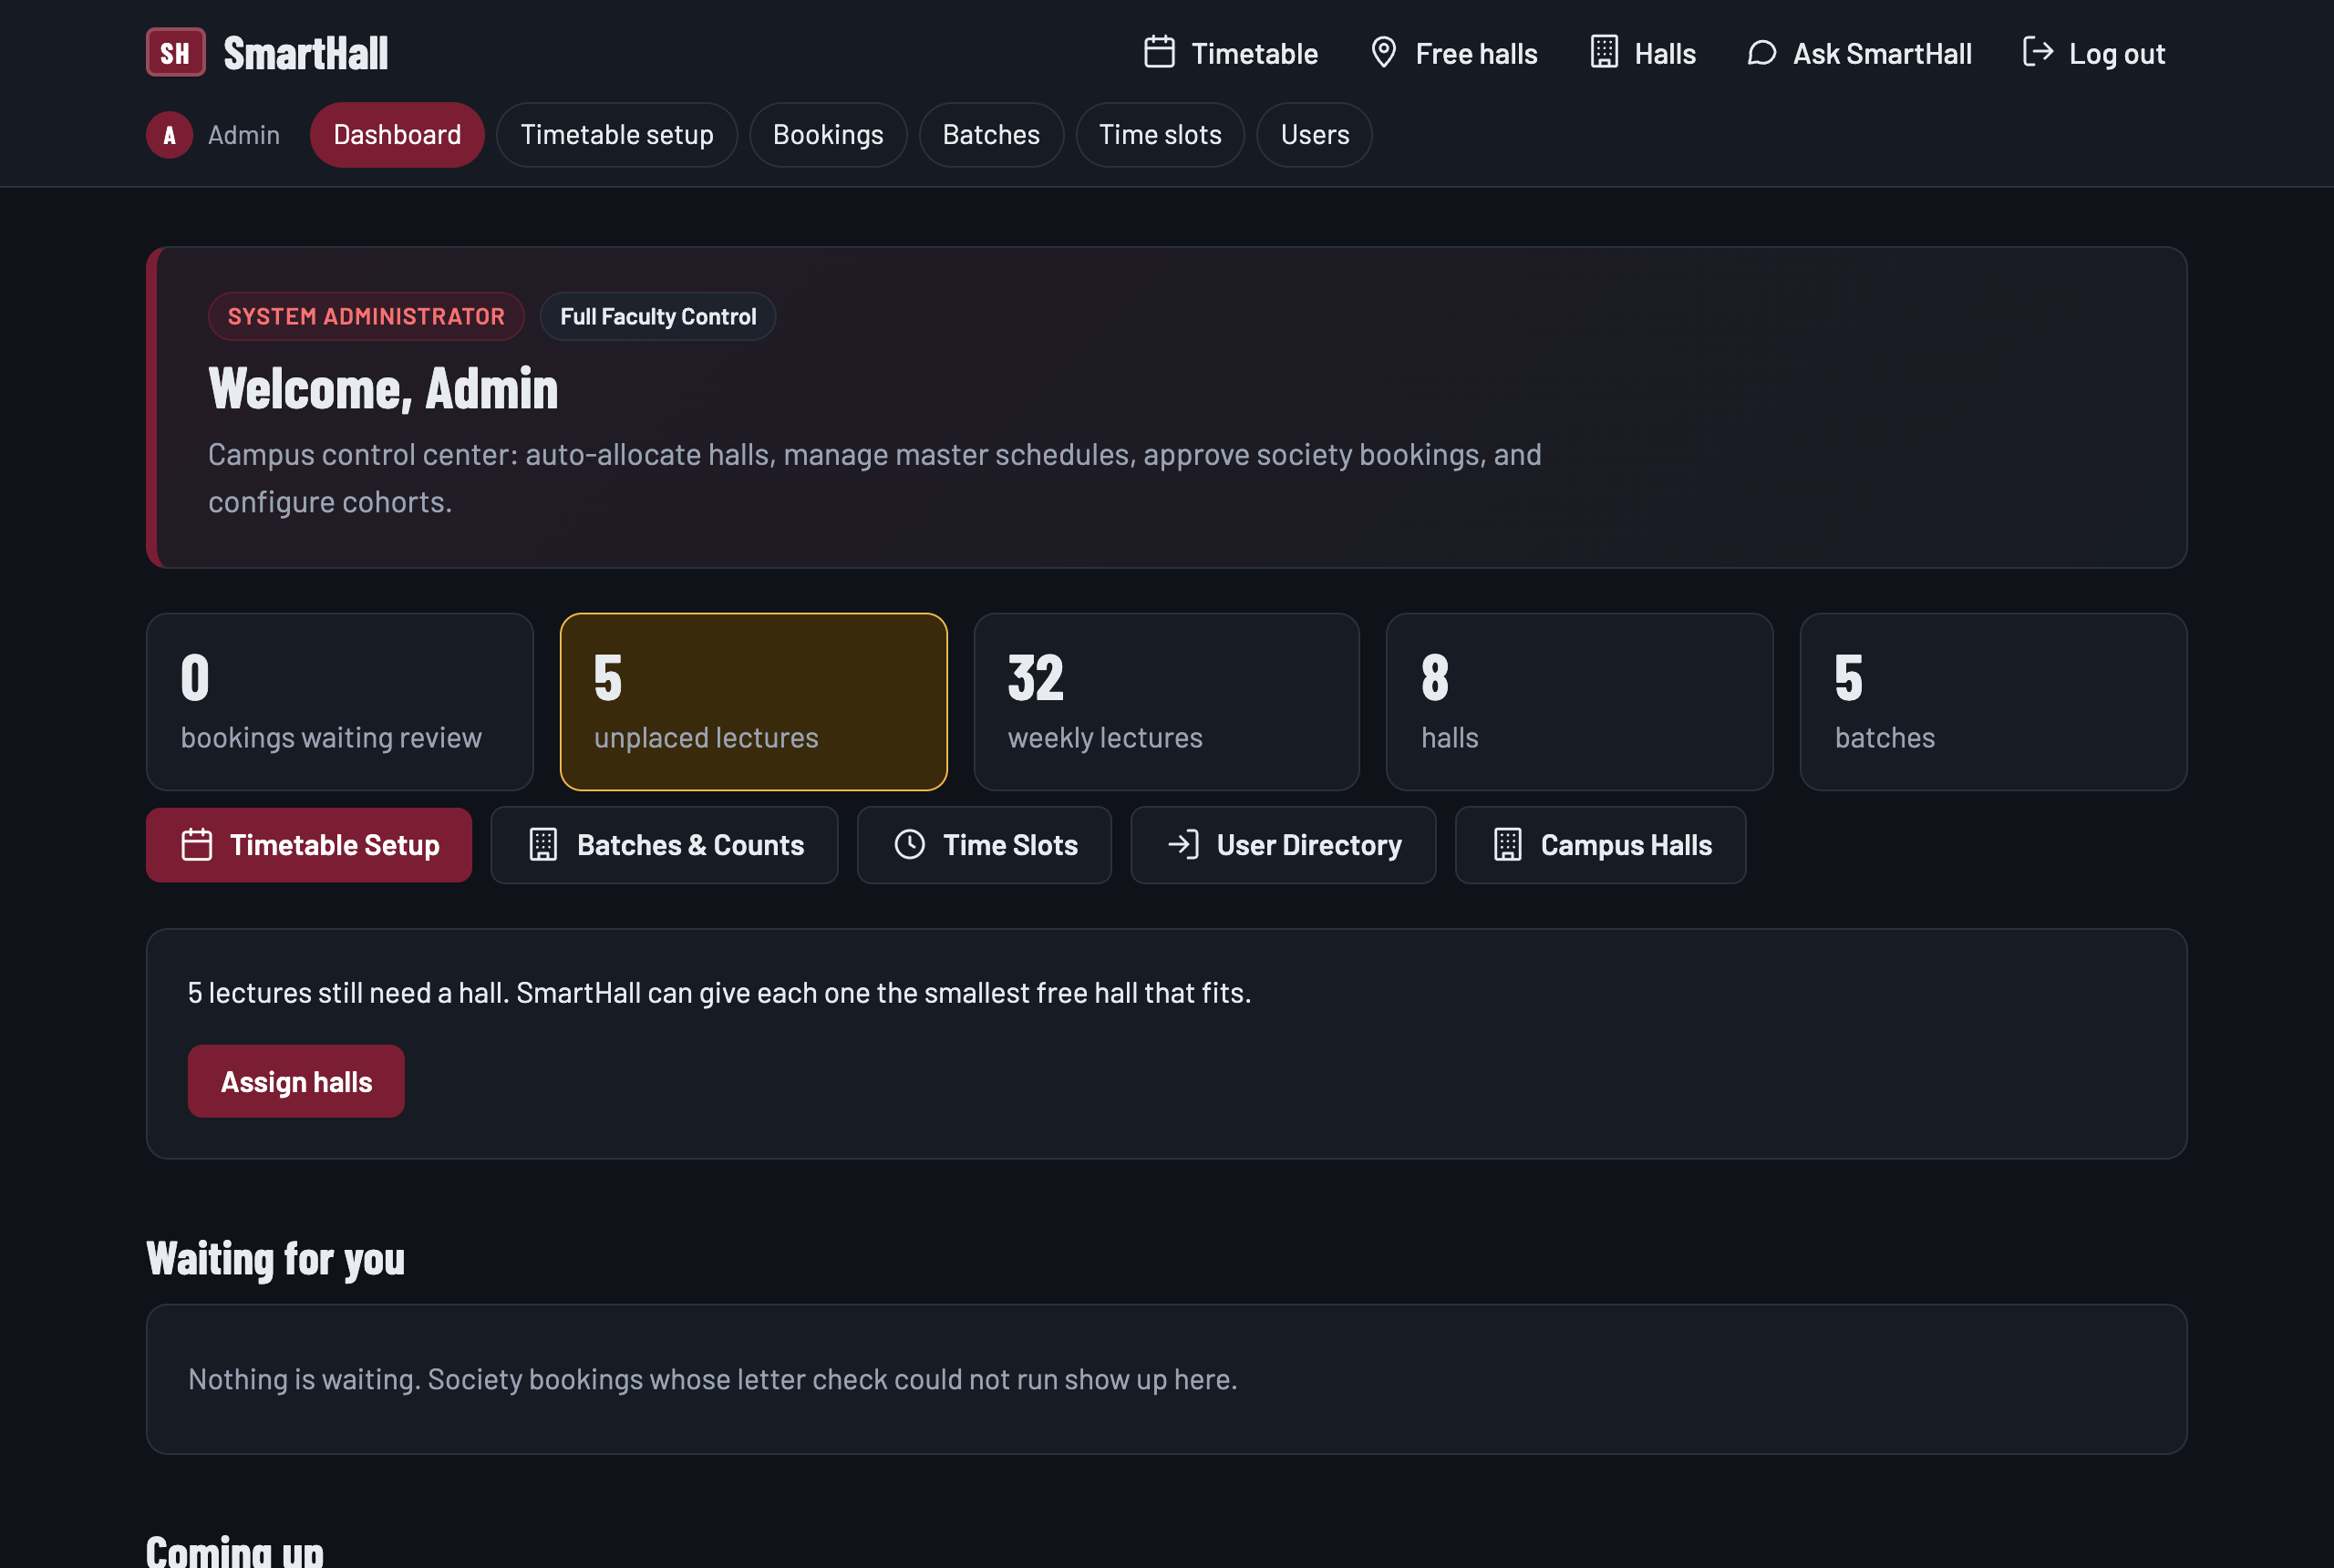
\includegraphics[width=0.95\textwidth]{report_assets/screenshots/admin_dashboard.png}
    \caption{Faculty Administrator Control Center (\texttt{/admin}) displaying active live stat tiles, pending approvals, and administrative shortcuts.}
    \label{fig:admin_dashboard}
\end{figure}

\newpage
\subsection{Batch Representative Workspace (\texttt{/rep})}
Dedicated dashboard for elected batch reps (e.g., \texttt{rep.e21@smarthall.test} for Batch 25 / E21):
\begin{itemize}
    \item \textbf{Enrolled Headcount Indicator:} Displays official cohort strength (e.g., \textit{210 students}), automatically enforced during room matching.
    \item \textbf{Today's Lecture Timeline:} Chronological list of day's classes with doorplate badges (\texttt{LH1}, \texttt{MLT}), times, and lecturers.
    \item \textbf{Next Lecture Tracker:} Real-time status card showing the class currently in session or up next with directions.
    \item \textbf{Matching Campus Halls:} Automatically highlights only venues accommodating the cohort headcount ($\ge 210$ seats).
    \item \textbf{Batch Timetable Management:} 1-click access to book extra tutorial slots or adjust the batch's weekly schedule.
\end{itemize}

\begin{figure}[H]
    \centering
    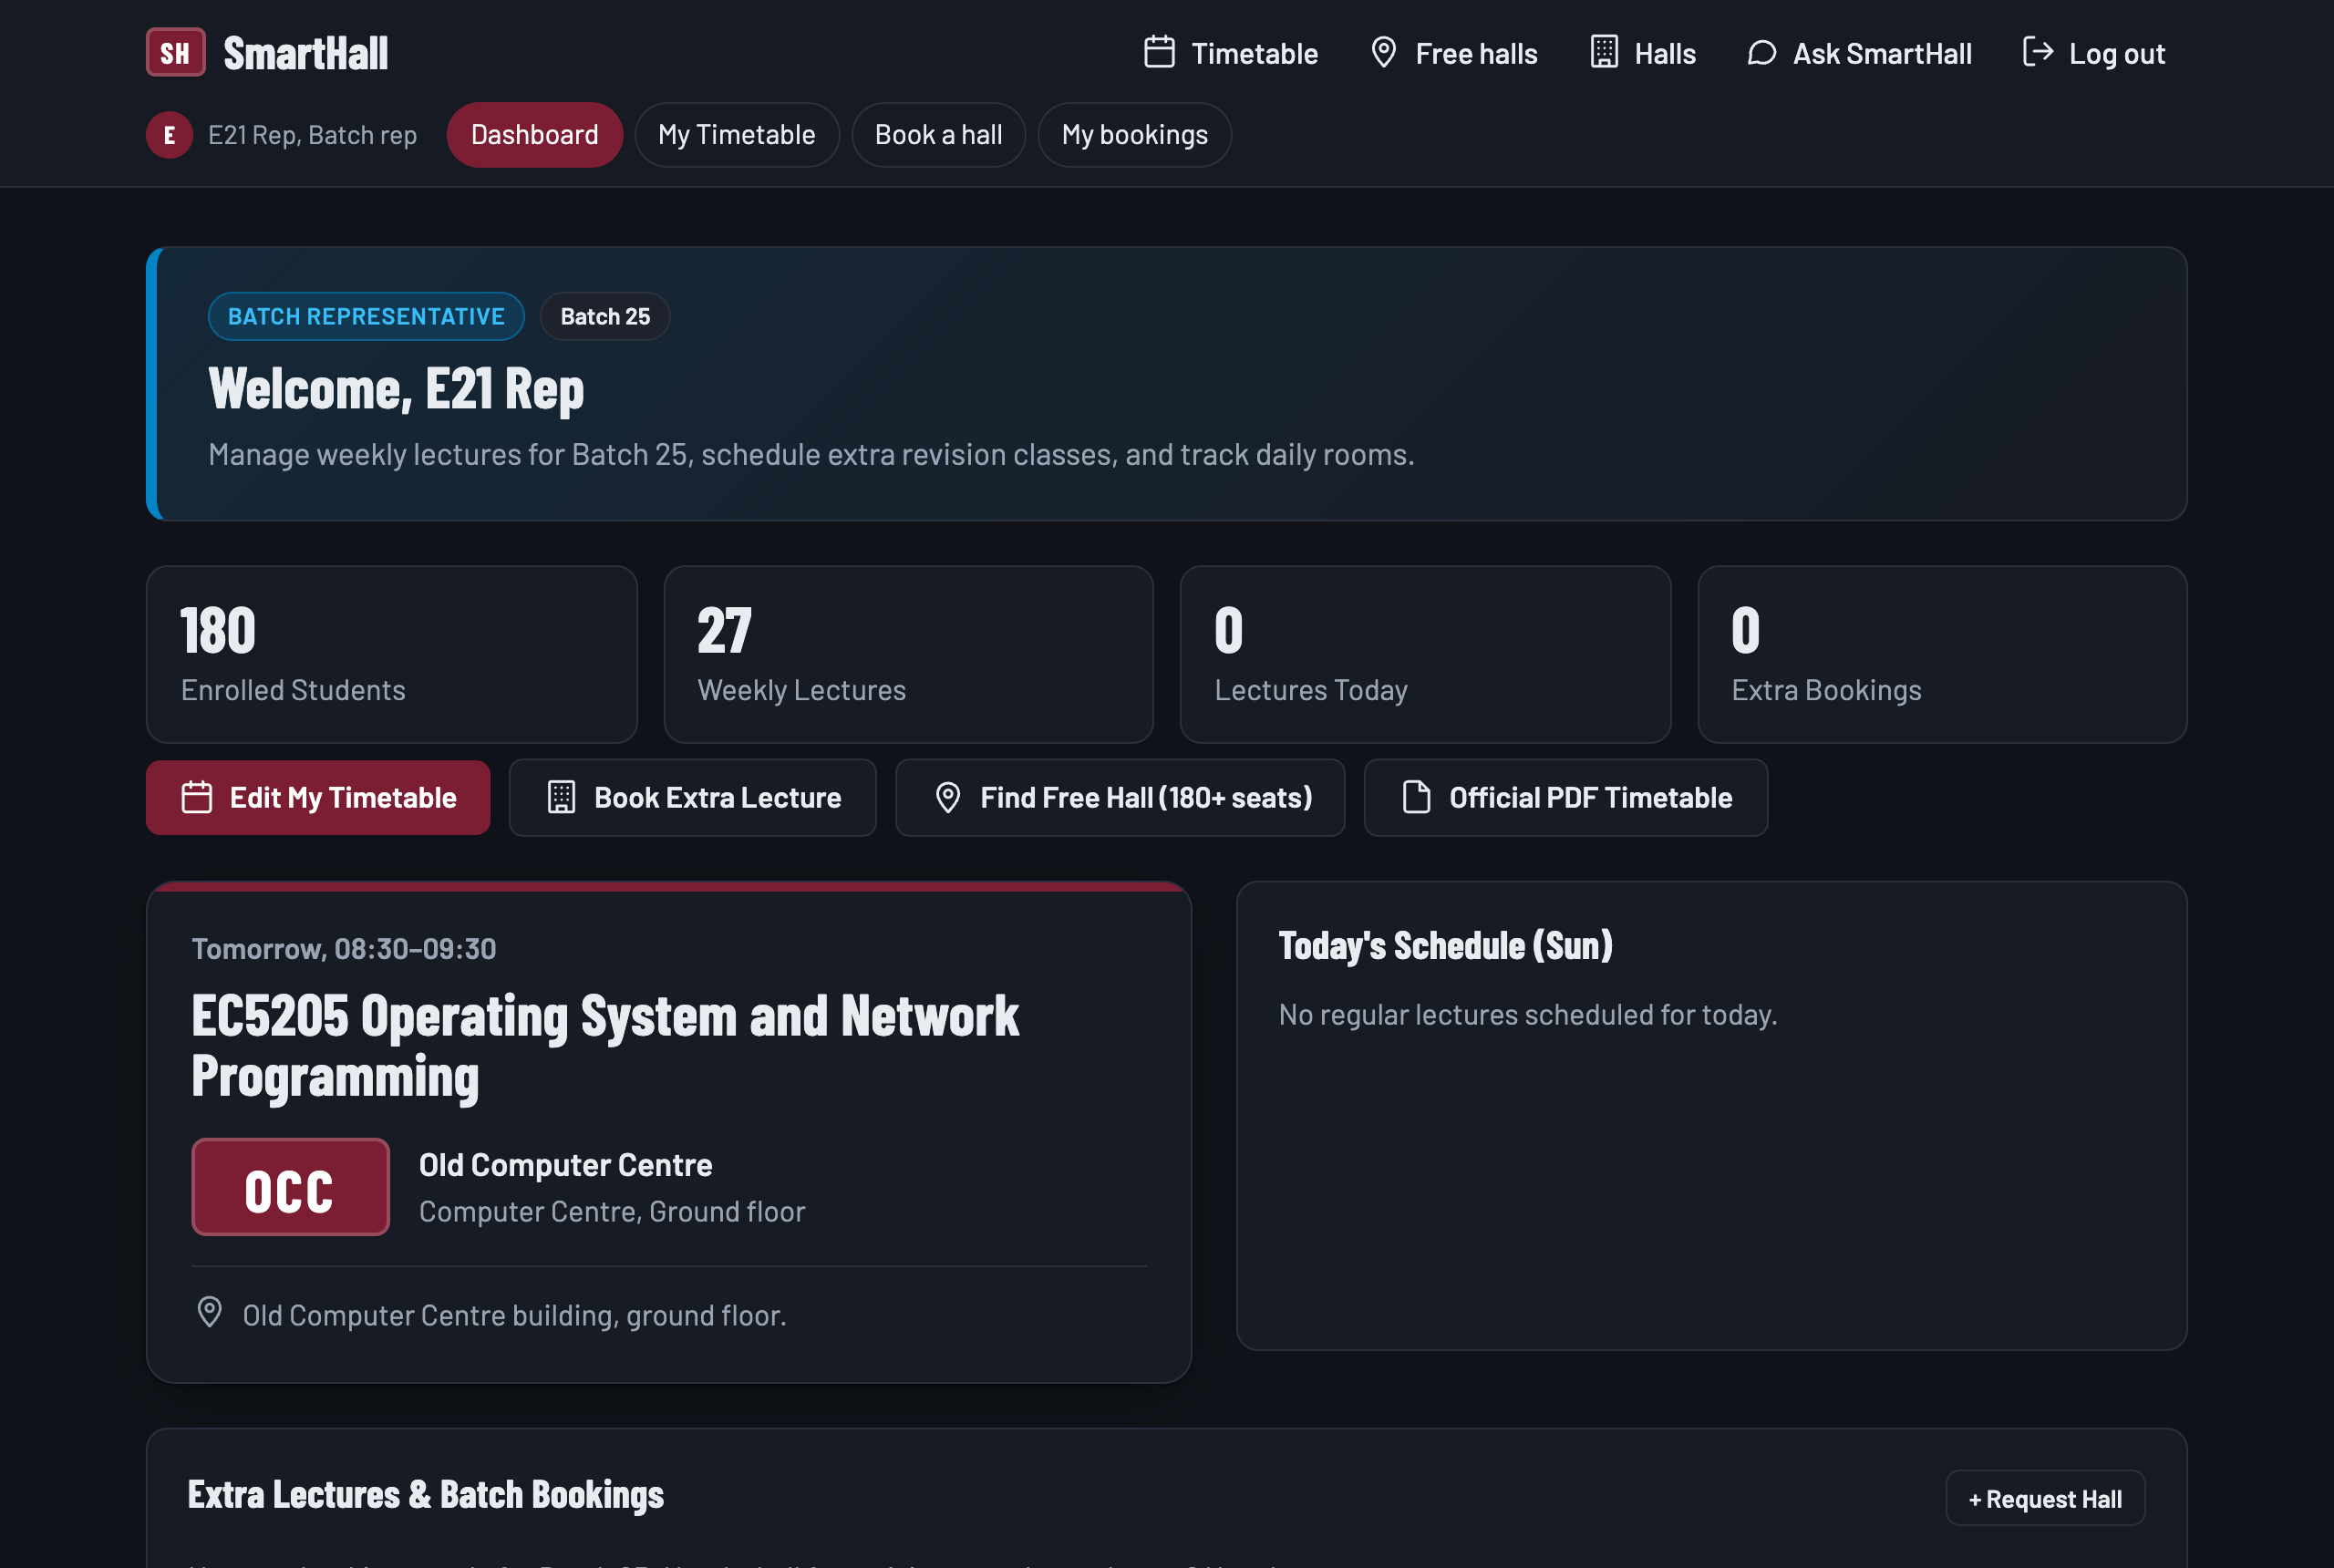
\includegraphics[width=0.95\textwidth]{report_assets/screenshots/rep_dashboard.png}
    \caption{Batch Representative Workspace (\texttt{/rep}) showing enrolled cohort strength (210 students), today's lecture schedule, live next-lecture indicator, and fitting halls.}
    \label{fig:rep_dashboard}
\end{figure}

\newpage
\subsection{Society President Portal (\texttt{/president})}
Event booking and compliance management for student organizations (e.g., \texttt{ieee@smarthall.test} for IEEE Student Branch):
\begin{itemize}
    \item \textbf{Reservation Pipeline Metrics:} 4-metric tracker for Total Requests, Confirmed Venues, In Review, and Rejected events.
    \item \textbf{AI Letter Compliance Guidelines:} Clear instructions on the 6 verification rules evaluated by Claude Opus (Letterhead, Addressee, Counselor Signatures).
    \item \textbf{Decision Logs \& Booking Audit:} Full status history showing requested venue, date, time slot, and AI rationale notes.
    \item \textbf{Auditorium Showcase:} Dedicated venue cards for large gathering spaces (\texttt{MLT}, \texttt{AUD}, \texttt{DO}) with capacities.
\end{itemize}

\begin{figure}[H]
    \centering
    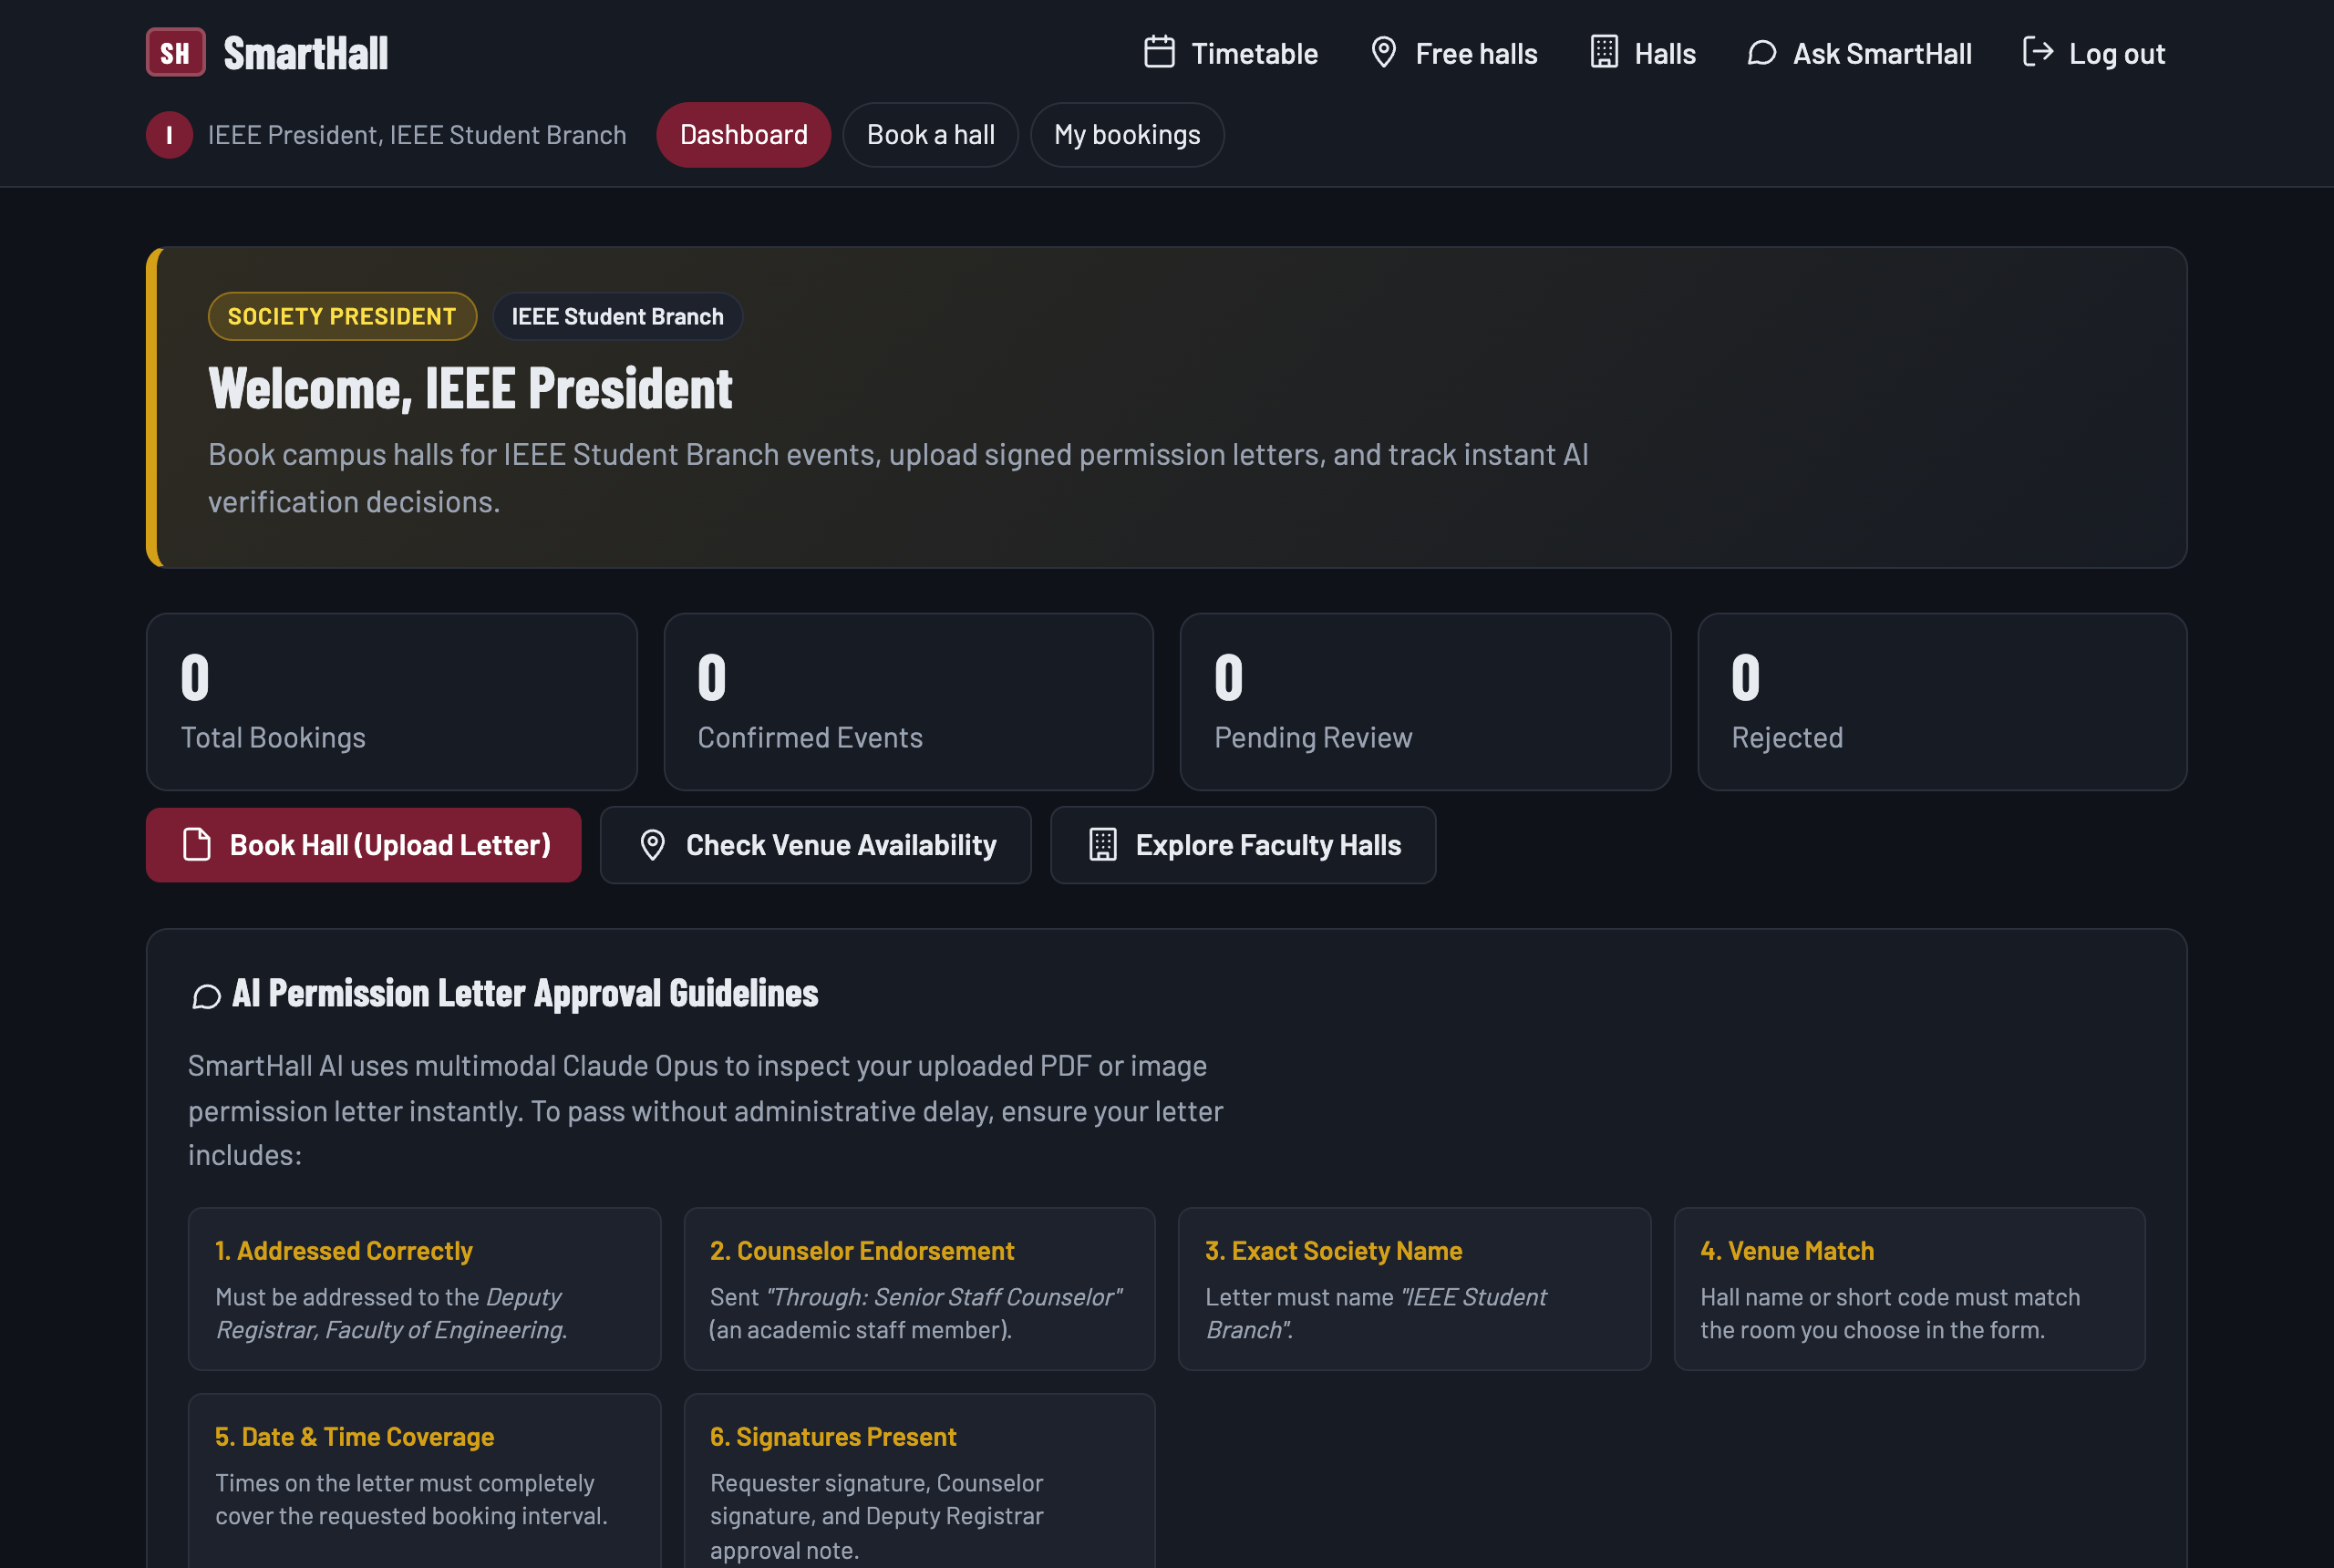
\includegraphics[width=0.95\textwidth]{report_assets/screenshots/president_portal.png}
    \caption{Society President Portal (\texttt{/president}) featuring event reservation metrics, AI permission letter compliance guidelines, and large auditorium showcase.}
    \label{fig:president_portal}
\end{figure}

% ----------------- SECTION 8 & 9 -----------------
\section{Custom Confirmation Modal UI}
Rather than relying on browser-native \texttt{window.confirm()} popups (which are unstyled and interrupt the main JavaScript thread), SmartHall AI implements an HTML5 \texttt{<dialog>} modal:
\begin{itemize}
    \item \textbf{Dark Glass Backdrop:} Semi-transparent overlay with \texttt{backdrop-filter: blur(8px)}.
    \item \textbf{Contextual Danger Indicators:} Circular red badge with trash SVG icon and explicit deletion details (e.g., \textit{"Are you sure you want to delete 'IS2101 Mathematics' for 27 (Mon 08:00--10:00)?"}).
    \item \textbf{Accessibility:} Full keyboard trapping, \texttt{Esc} key dismissal, and backdrop click-to-close.
    \item \textbf{Universal Safeguard:} Protects timetable entries, batches, time slots, campus halls, bookings, and semester resets.
\end{itemize}

\section{Conclusion}
SmartHall AI demonstrates how modern, lightweight web technologies and targeted AI integrations can solve real-world logistical bottlenecks in higher education institutions. By harmonizing algorithmic allocation, automated document parsing, multimodal AI verification, dedicated role-based interfaces, and an intentional user interface, the system provides the Faculty of Engineering, University of Ruhuna, with a dependable, state-of-the-art campus infrastructure management platform.

\end{document}
